\documentclass[a4paper]{article}
\usepackage{mystyle}

\begin{document}

\customtitle{Fluctuation Strength Test Battery Specification}

\section{Introduction}

This document details a series of test that will be used to validate our
fluctuation strength model. These tests will be based on the reference value of
fluctuation strength and its the parametric dependencies. For all the tests a
sampling frequency $f_s = 44100 $ Hz will be used.

\section{Reference Value}

An amplitude-modulated (AM) tone ($f_c = 1$ kHz, $f_m = 4$ Hz, $m_d = 1$,
SPL $=60$ dB) is assigned a fluctuation strength of 1 vacil, and thus
constitutes the reference value. As so, the model implementation must comply
with this requisite.

\section{Tests}

This section details the specific tests that the model must pass to be
considered adequate. According to the type of input stimuli different tests
will be specified, starting with AM tones and then expanding to
frequency-modulated (FM) tones and AM broadband noise (BBN).

\subsection{AM Tones}

\subsubsection{Modulation Frequency}

The most characteristic attribute of fluctuation strength is its bandpass
response with regard to the variation of the modulation frequency (Figure
\ref{fig:flucstrenvmodfreq}b). As so, this particular plot will be reproduced
using the input stimuli whose parameters are shown on Listing
\ref{lst:amparamsfmplot}.

\begin{lstlisting}[
    style=MATLAB-editor,
    caption={AM tones parameters modulation frequency plot},
    label={lst:amparamsfmplot}
]
fc  = 1000; % [Hz]
md  = 40; % [dB]
SPL = 70; % [dB]
fs  = 44100; % [Hz]
FMs = [0 0.25 0.50 1.00 2.00 4.00 8.00 16.00 32.00]; % [Hz]
\end{lstlisting}

\begin{figure}[ht]
    \centering
    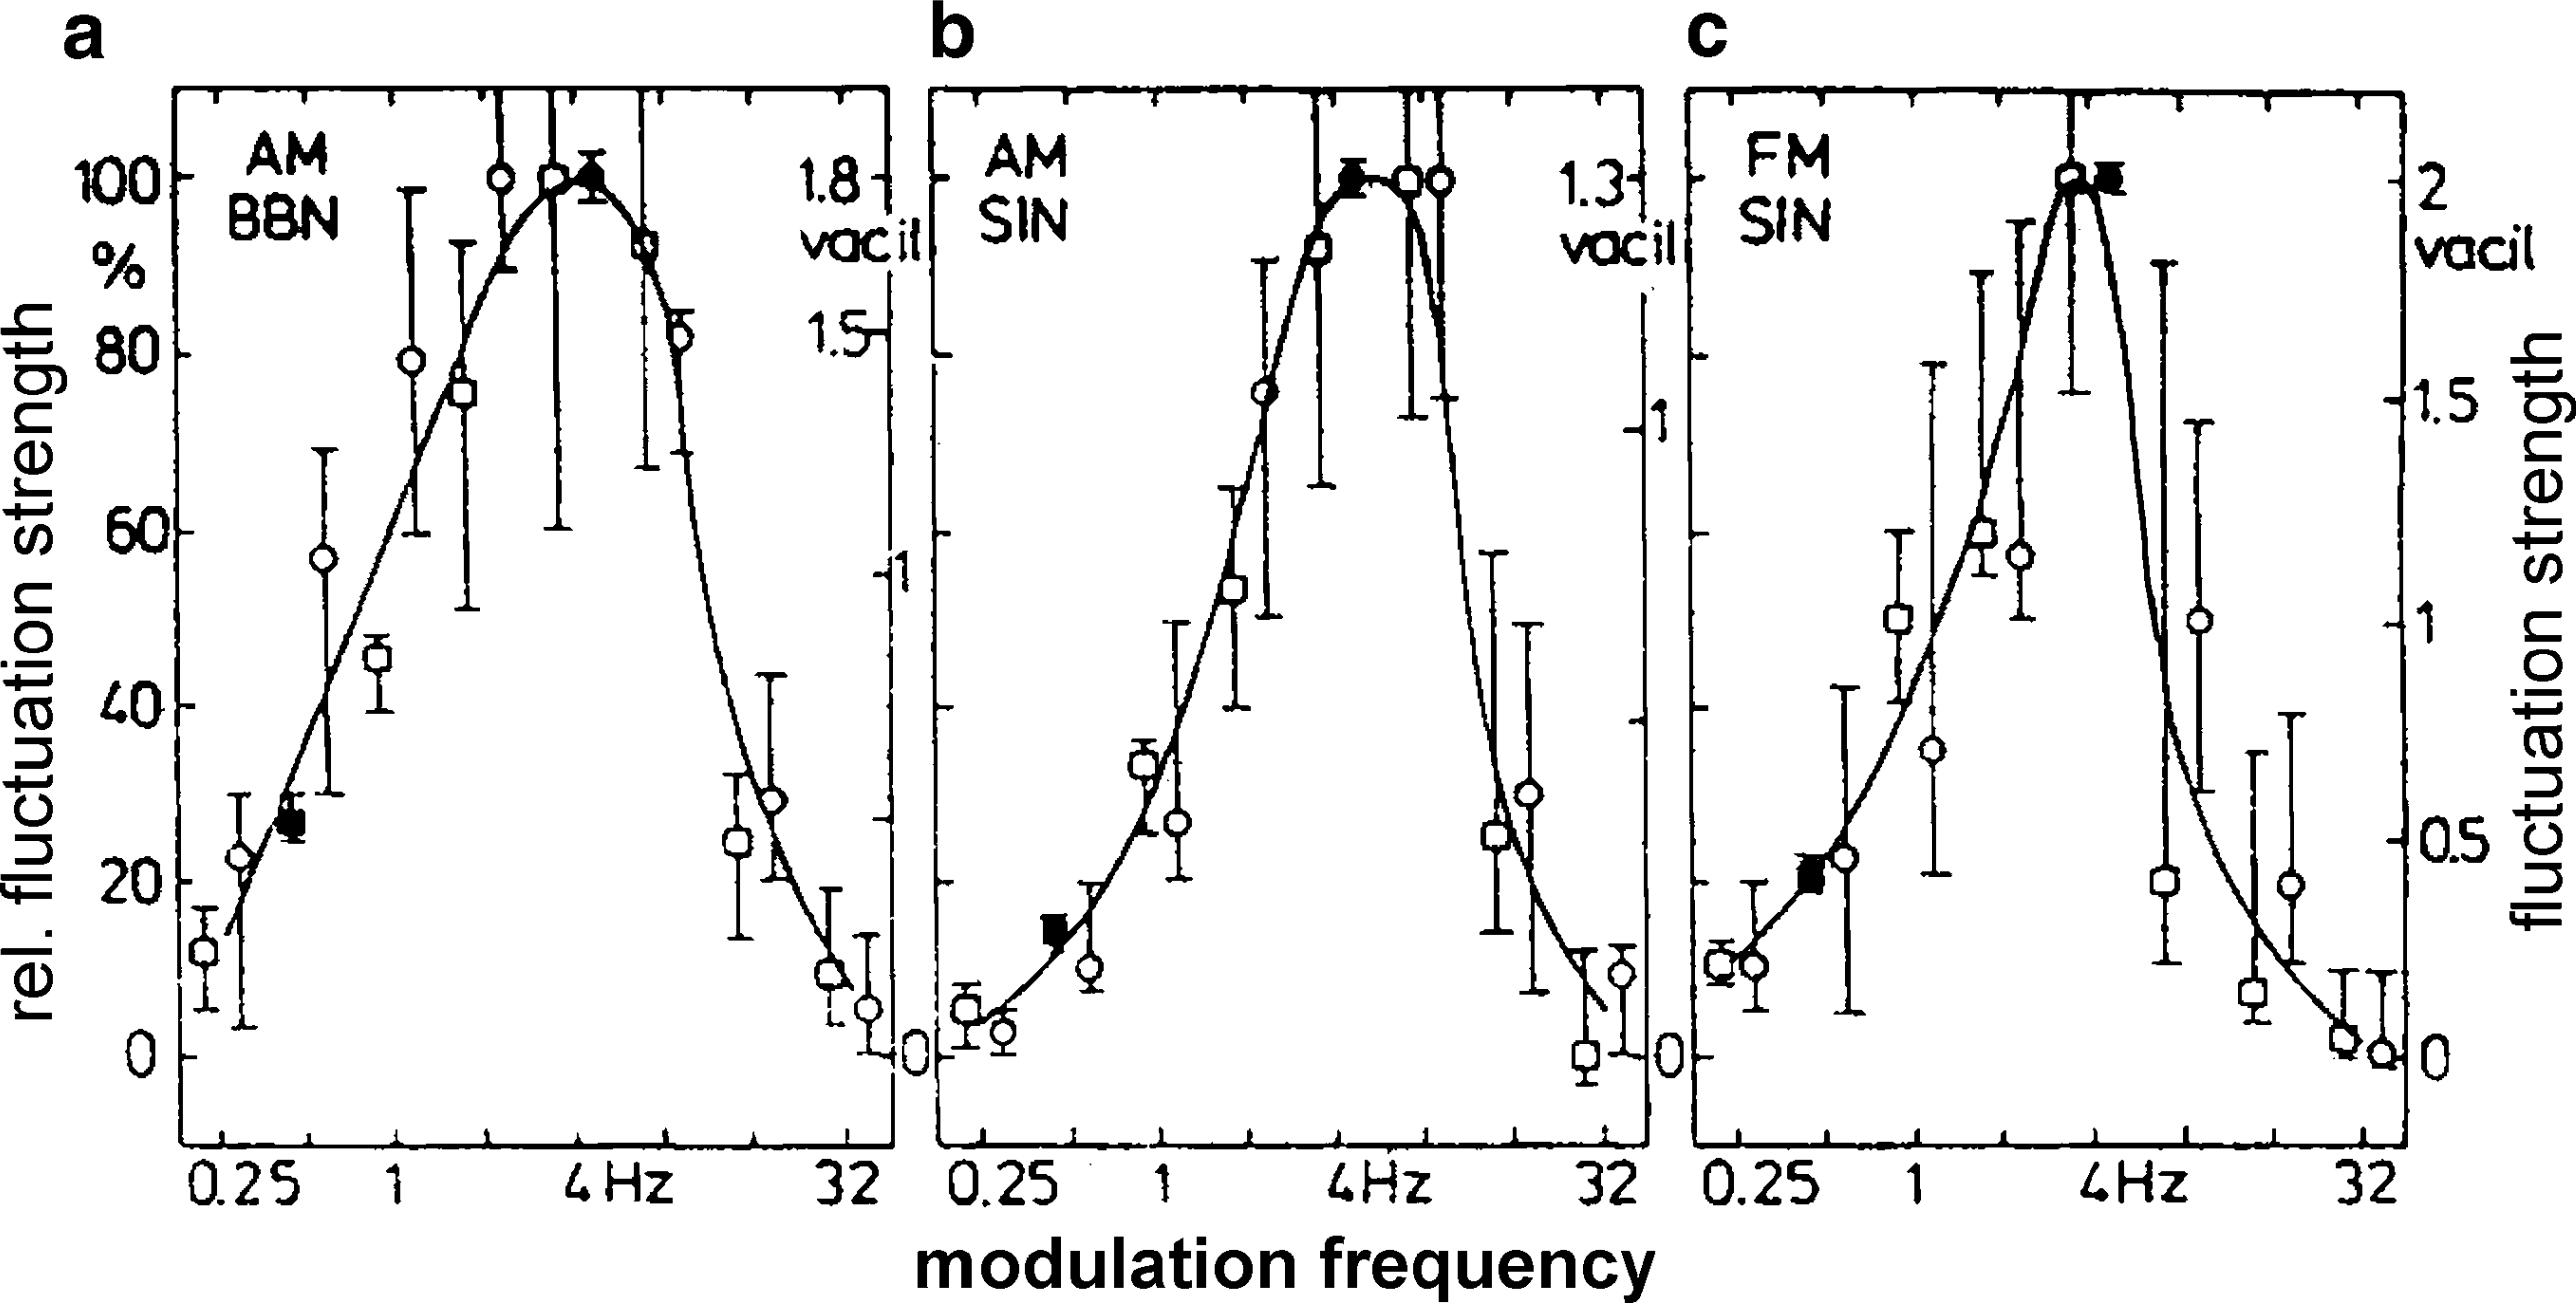
\includegraphics[height=8cm]
        {Mueller2012Handbook/img/FluctuationStrengthVsModulationFrequency}
    \caption{Fluctuation strength of three modulated sounds as a function of
        modulation frequency. (a) Amplitude-modulated broad-band noise of 60-dB
        SPL and 40-dB modulation depth; (b) amplitude-modulated 1-kHz tone of
        70-dB SPL and 40-dB modulation depth; (c) frequency-modulated pure tone
        of 70-dB SPL, 1500-Hz center frequency and $\pm$ 700-Hz frequency
        deviation~\cite[pp. 248]{Fastl2007Psychoacoustics}}
\label{fig:flucstrenvmodfreq}
\end{figure}

\subsection{Carrier Frequency}

In the implementation of \citeauthor{Schrader2002}, the parameter
\matlabinline{gzi} is used to model the dependency of roughness on the carrier
frequency. In order to evaluate whether the proposed values hold, and whether
it is necessary to adjust them, Figure~\ref{fig:flucstrenvscfreq}a will be used.
The input stimuli parameters to be used are listed in Listing
\ref{lst:amparamsfcplot}.

\begin{lstlisting}[
    style=MATLAB-editor,
    caption={AM tones parameters carrier frequency plot},
    label={lst:amparamsfcplot}
]
FCs = [125 250 500 1000 2000 4000 8000]; % [Hz]
md  = 40; % [dB]
SPL = 70; % [dB]
fs  = 44100; % [Hz]
fm  = 4; % [Hz]
\end{lstlisting}

\begin{figure}[ht]
    \centering
    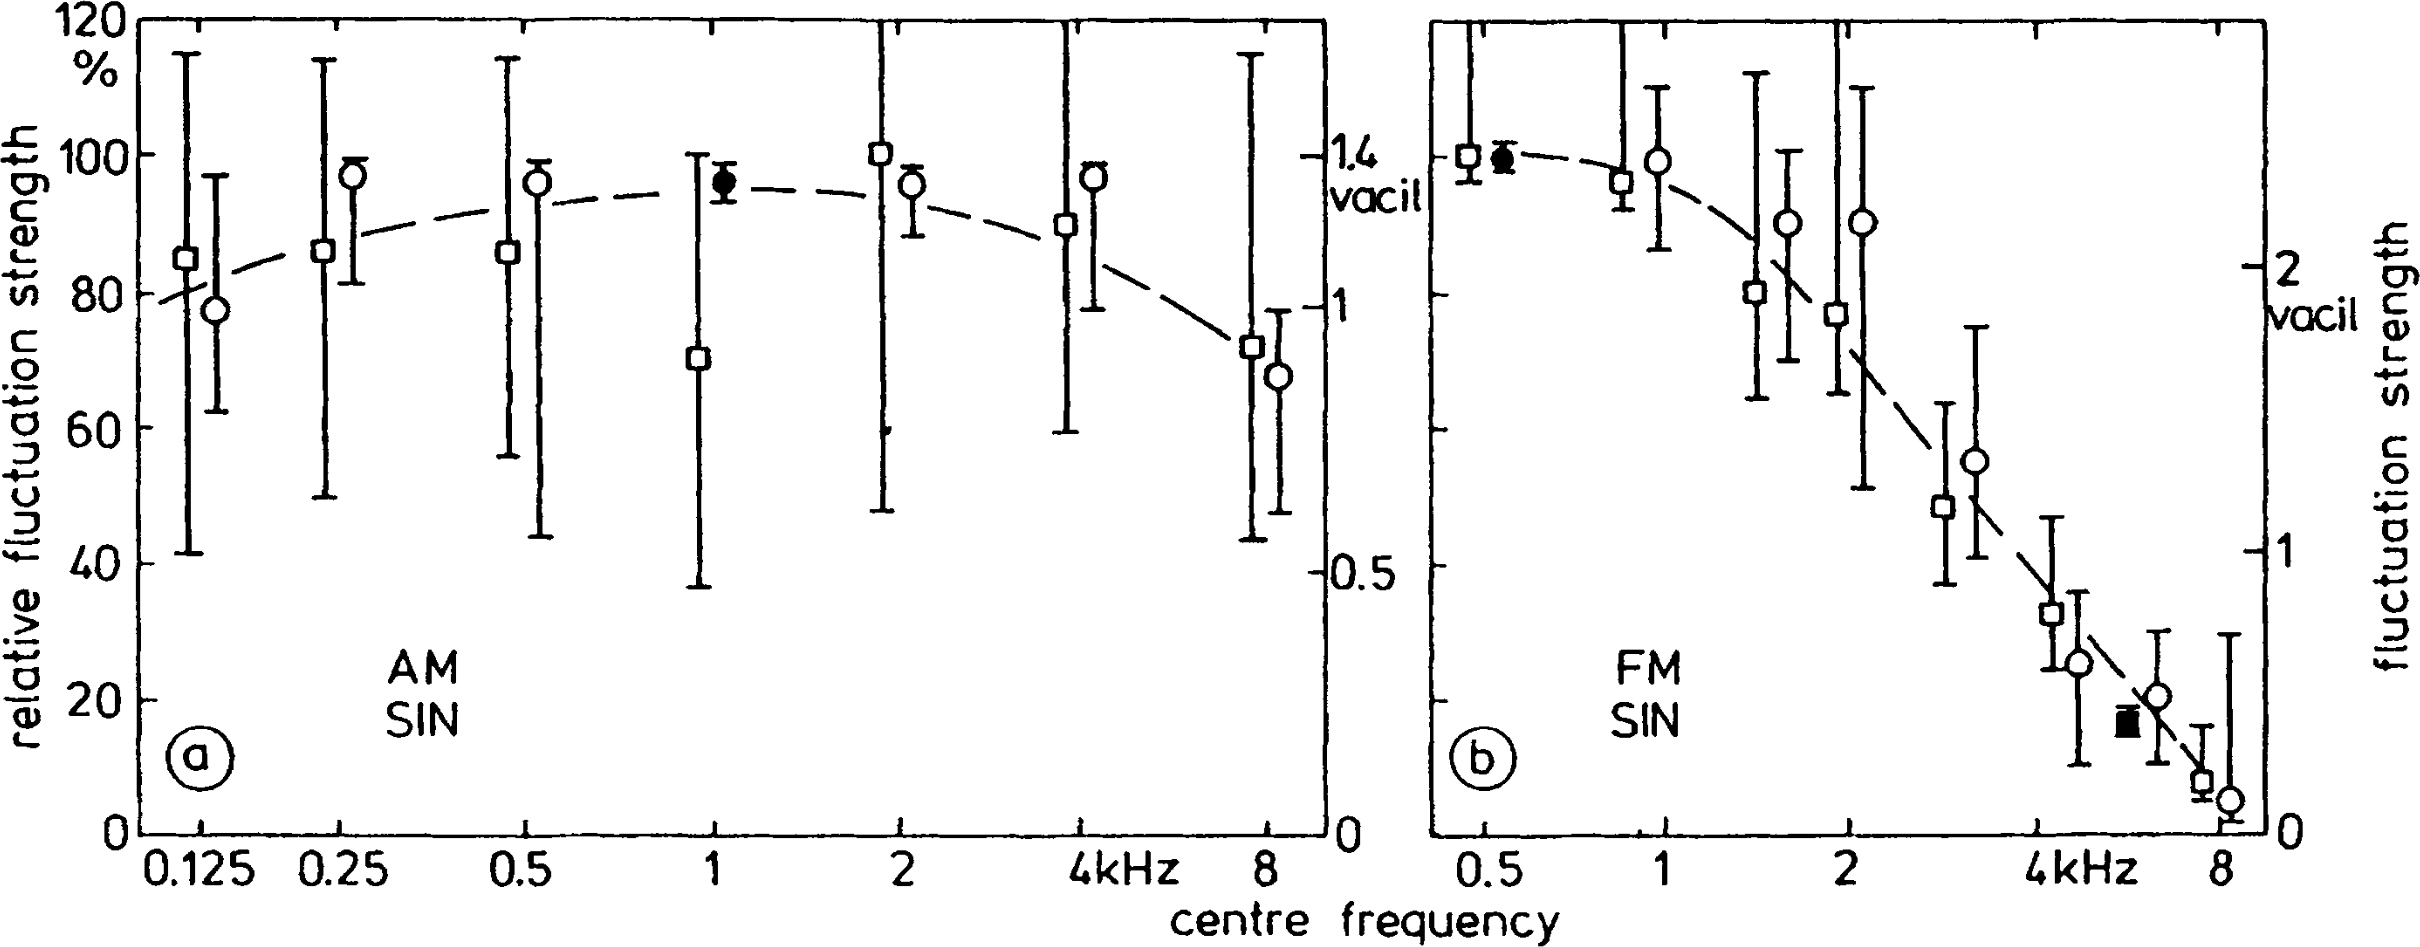
\includegraphics[height=5cm]
        {Fastl2007Psychoacoustics/img/FluctuationStrengthVsCenterFrequency}
    \caption{Fluctuation strength of modulated tones as a function of
        frequency. (a) Amplitude-modulated pure tone of 70-dB SPL, 4-Hz
        modulation frequency and 40-dB modulation depth; (b)
        frequency-modulated pure tone of 70-dB SPL, 4-Hz modulation frequency,
        and ±200-Hz frequency
        deviation~\cite[pp. 250]{Fastl2007Psychoacoustics}}
\label{fig:flucstrenvscfreq}
\end{figure}

\subsection{Sound Pressure Level}

Figure~\ref{fig:flucstrenvsndpreslvl} will be reproduced using the stimuli whose
parameters are shown in Listing~\ref{lst:amparamssplplot};

\begin{lstlisting}[
    style=MATLAB-editor,
    caption={AM tones parameters sound pressure level plot},
    label={lst:amparamssplplot}
]
FCs     = 1000; % [Hz]
md      = 40; % [dB]
SPLs    = [50 60 70 80 90]; % [dB]
fs      = 44100; % [Hz]
fm      = 4; % [Hz]
\end{lstlisting}

\begin{figure}[ht]
    \centering
    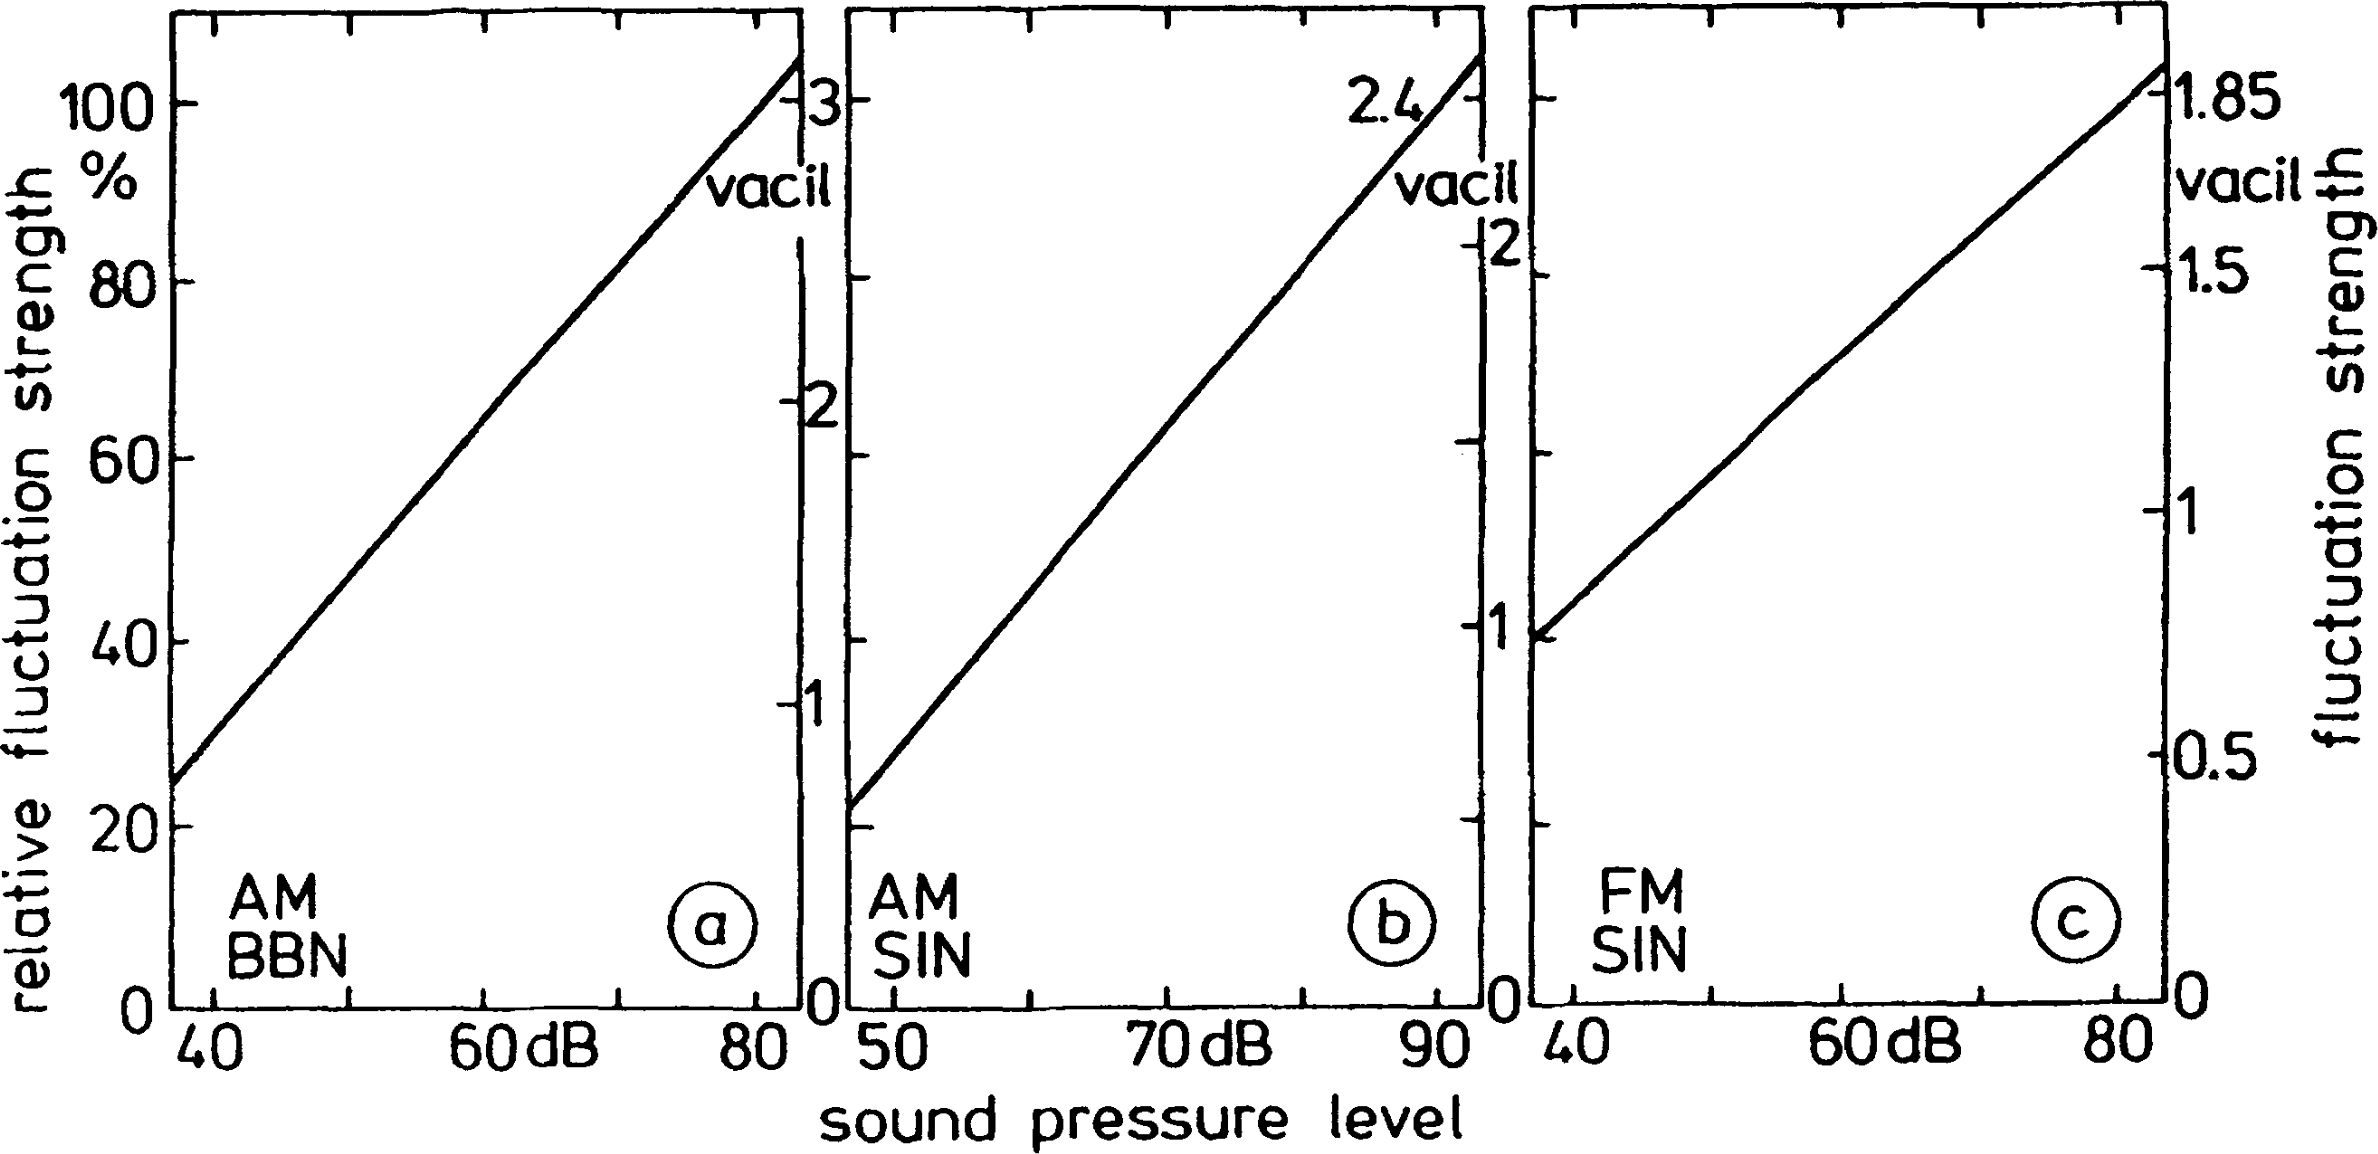
\includegraphics[height=5cm]
        {Fastl2007Psychoacoustics/img/FluctuationStrengthVsSoundPressureLevel}
    \caption{Fluctuation strength of modulated sounds as a function of sound
        pressure level. Stimulus parameters are the same as in
        Figure~\ref{fig:flucstrenvmodfreq}, but the modulation frequency is
        4Hz~\cite[pp. 249]{Fastl2007Psychoacoustics}}
\label{fig:flucstrenvsndpreslvl}
\end{figure}

\subsection{Modulation Depth}

Figure~\ref{fig:flucstrenvsmoddep} will be reproduced using the stimuli whose
parameters are presented in Listing~\ref{lst:amparamssmdplot}.

\begin{lstlisting}[
    style=MATLAB-editor,
    caption={AM tones parameters modulation depth plot},
    label={lst:amparamssmdplot}
]
FCs = 1000; % [Hz]
MDs = [1 2 4 6 8 12 16 20 40]; % [dB]
SPL = 70; % [dB]
fs  = 44100; % [Hz]
fm  = 4; % [Hz]
\end{lstlisting}

\begin{figure}[ht]
    \centering
    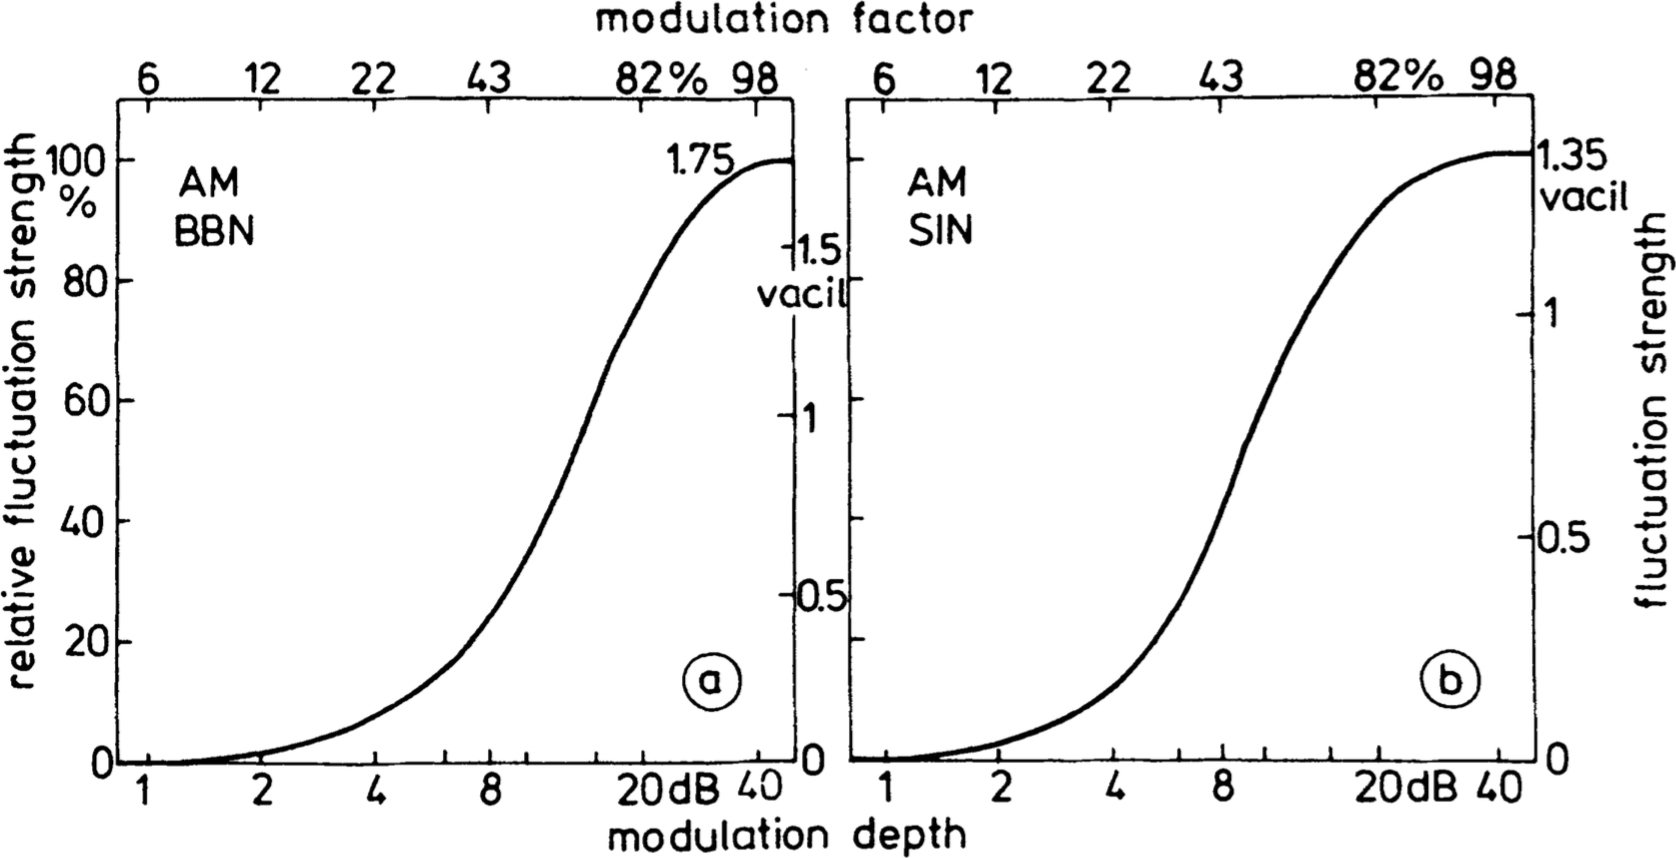
\includegraphics[height=5cm]
        {Fastl2007Psychoacoustics/img/FluctuationStrengthVsModulationDepth}
    \caption{Fluctuation strength of two amplitude-modulated sounds as a
        function of modulation depth (or modulation factor). (a)
        Amplitude-modulated broadband noise of 60-dB SPL and 4-Hz modulation
        frequency; (b) amplitude-modulated 1-kHz tone of 70-dB SPL and 4-Hz
        modulation frequency~\cite[pp. 249]{Fastl2007Psychoacoustics}}
\label{fig:flucstrenvsmoddep}
\end{figure}

\section{FM Tones}

\subsection{Modulation Frequency}

Figure~\ref{fig:flucstrenvmodfreq}c shows the dependency between modulation
frequency and fluctuation strength for FM tones. Listing
\ref{lst:fmparamsfmplot} describes the parameters of the test stimuli to use.

\begin{lstlisting}[
    style=MATLAB-editor,
    caption={FM tones parameters modulation frequency plot},
    label={lst:fmparamsfmplot}
]
fc  = 1500; % [Hz]
df  = 700; % [Hz]
SPL = 70; % [dB]
fs  = 44100; % [Hz]
FMs = [0 0.25 0.50 1.00 2.00 4.00 8.00 16.00 32.00]; % [Hz]
\end{lstlisting}

\subsection{Carrier Frequency}

Figure~\ref{fig:flucstrenvscfreq}b will be reproduced using the stimuli whose
parameters are presented in Listing~\ref{lst:fmparamsfcplot}.

\begin{lstlisting}[
    style=MATLAB-editor,
    caption={FM tones parameters carrier frequency plot},
    label={lst:fmparamsfcplot}
]
FCs = [500 1000 1500 2000 3000 4000 6000 8000]; % [Hz]
df  = 200; % [Hz]
SPL = 70; % [dB]
fs  = 44100; % [Hz]
fm  = 4; % [Hz]
\end{lstlisting}

\subsection{Sound Pressure Level}

Figure~\ref{fig:flucstrenvsndpreslvl}c will be reproduced using the stimuli
whose parameters are presented in Listing~\ref{lst:fmparamssplplot}.

\begin{lstlisting}[
    style=MATLAB-editor,
    caption={FM tones parameters sound pressure level plot},
    label={lst:fmparamssplplot}
]
fc      = 1500; % [Hz]
df      = 700; % [Hz]
SPLs    = [40 50 60 70 80]; % [dB]
fs      = 44100; % [Hz]
fm      = 4; % [Hz]
\end{lstlisting}

\subsection{Frequency Deviation}

Figure~\ref{fig:flucstrenvfreqdev} will be reproduced using the stimuli whose
parameters are presented in Listing~\ref{lst:fmparamsfreqdevplot}.

\begin{figure}[ht]
    \centering
    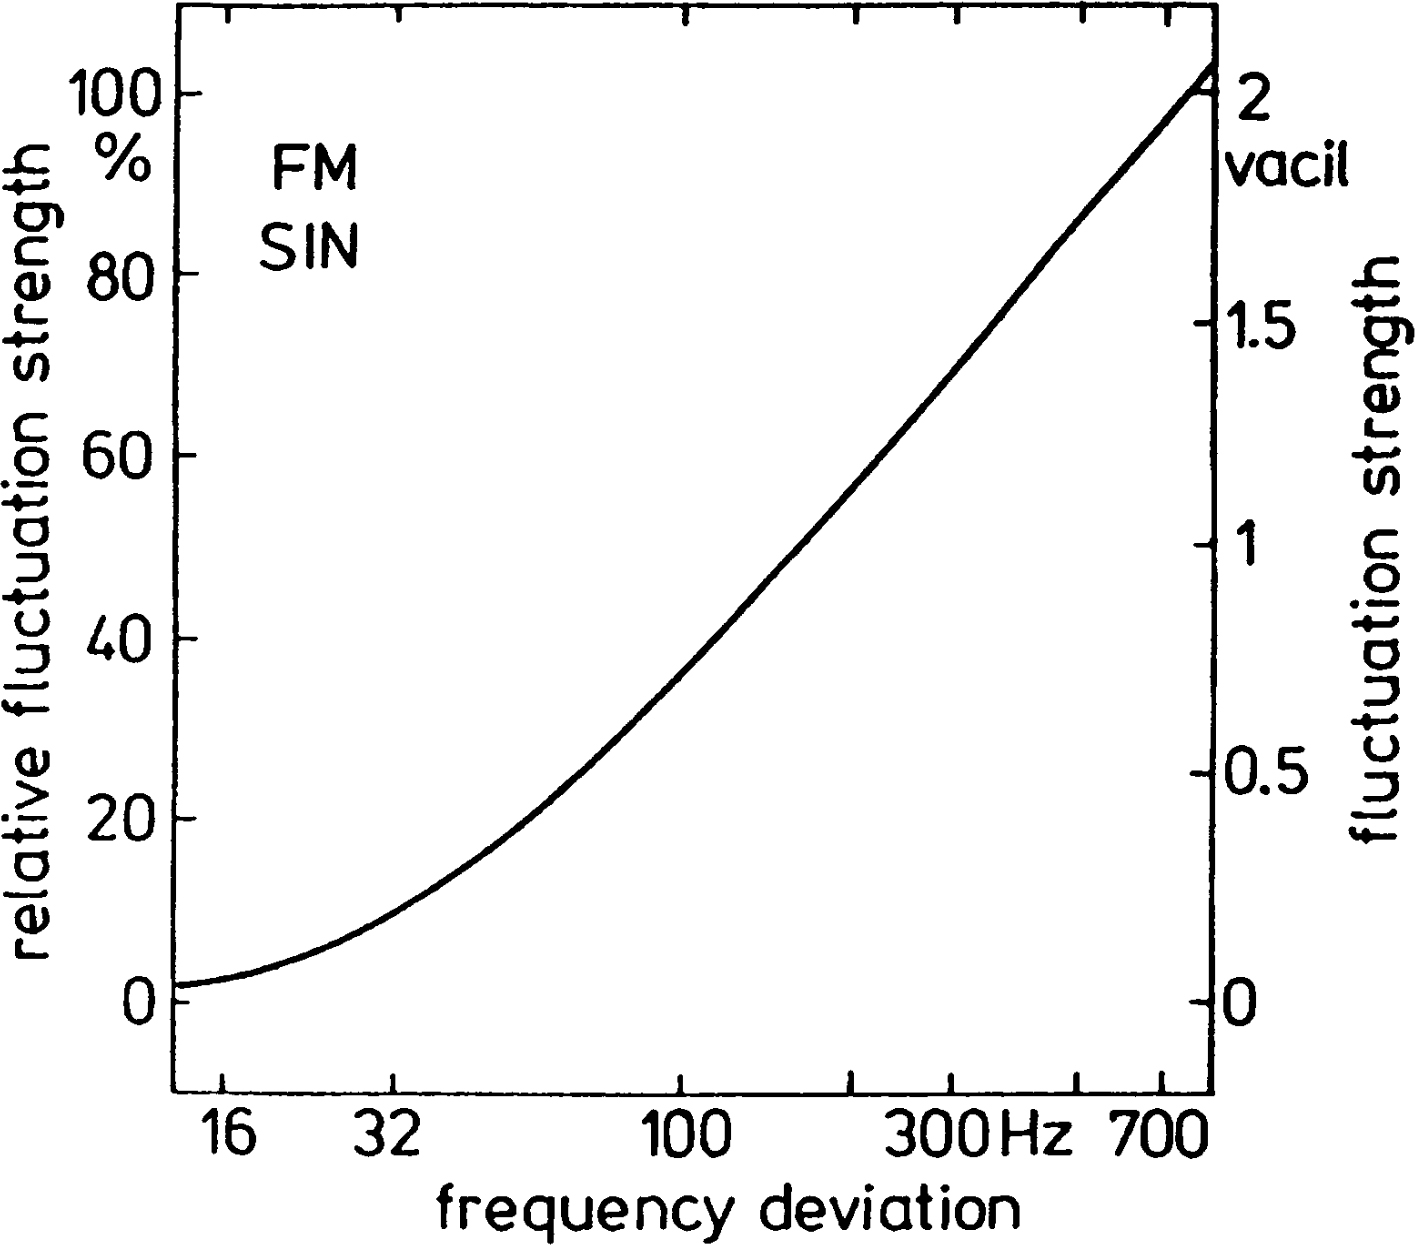
\includegraphics[height=5cm]
        {Fastl2007Psychoacoustics/img/FluctuationStrengthVsFrequencyDeviation}
    \caption{Fluctuation strength as a function of frequency deviation for a
        tone with 70 dB SPL, 1.5 kHz center frequency and a modulation frequency
        of 4 Hz~\cite[pp. 251]{Fastl2007Psychoacoustics}}
\label{fig:flucstrenvfreqdev}
\end{figure}

\begin{lstlisting}[
    style=MATLAB-editor,
    caption={FM tones parameters frequency deviation plot},
    label={lst:fmparamsfreqdevplot}
]
fc      = 1500; % [Hz]
DFs     = [16 32 100 300 700]; % [Hz]
SPL     = 70; % [dB]
fs      = 44100; % [Hz]
fm      = 4; % [Hz]
\end{lstlisting}

\custombibliography{}

\end{document}
